% Autor: Leonhard Segger, Alexander Neuwirth
% Datum: 2017-10-30
\documentclass[
	% Papierformat
	a4paper,
	% Schriftgröße (beliebige Größen mit „fontsize=Xpt“)
	12pt,
	% Schreibt die Papiergröße korrekt ins Ausgabedokument
	pagesize,
	% Sprache für z.B. Babel
	ngerman
]{scrartcl}

% Achtung: Die Reihenfolge der Pakete kann (leider) wichtig sein!
% Insbesondere sollten (so wie hier) babel, fontenc und inputenc (in dieser
% Reihenfolge) als Erstes und hyperref und cleveref (Reihenfolge auch hier
% beachten) als Letztes geladen werden!

\usepackage{tikz}
\usetikzlibrary{calc,patterns,angles,quotes} % loads some tikz extensions\usepackage{tikz}
\usetikzlibrary{babel}

% Silbentrennung etc.; Sprache wird durch Option bei \documentclass festgelegt
\usepackage{babel}
% Verwendung der Zeichentabelle T1 (Sonderzeichen etc.)
\usepackage[T1]{fontenc}
% Legt die Zeichenkodierung der Eingabedatei fest, z.B. UTF-8
\usepackage[utf8]{inputenc}
% Schriftart
\usepackage{lmodern}
% Zusätzliche Sonderzeichen
\usepackage{textcomp}

% Mathepaket (intlimits: Grenzen über/unter Integralzeichen)
\usepackage[intlimits]{amsmath}
% Ermöglicht die Nutzung von \SI{Zahl}{Einheit} u.a.
\usepackage{siunitx}
% Zum flexiblen Einbinden von Grafiken (\includegraphics)
\usepackage{graphicx}
% Abbildungen im Fließtext
\usepackage{wrapfig}
% Abbildungen nebeneinander (subfigure, subtable)
\usepackage{subcaption}
% Funktionen für Anführungszeichen
\usepackage{csquotes}
\MakeOuterQuote{"}
% Zitieren, Bibliografie
\usepackage[sorting=none]{biblatex}


% Zur Darstellung von Webadressen
\usepackage{url}
%chemische Formeln
\usepackage[version=4]{mhchem}
% siunitx: Deutsche Ausgabe, Messfehler getrennt mit ± ausgeben
\usepackage{floatrow}
\floatsetup[table]{capposition=top}
\usepackage{float}
% Verlinkt Textstellen im PDF-Dokument
\usepackage[unicode]{hyperref}
% "Schlaue" Referenzen (nach hyperref laden!)
\usepackage{cleveref}
\sisetup{
	locale=DE,
	separate-uncertainty
}
\bibliography{BA-C-04_MI_19-11-2018_References}

\begin{document}

	\begin{titlepage}
		\centering
		{\scshape\LARGE Versuchsbericht zu \par}
		\vspace{1cm}
		{\scshape\huge MI - Michelson-Interferometer \par} %TODO fine?
		\vspace{2.5cm}
		{\LARGE Gruppe BA-C-04 \par}
		\vspace{0.5cm}

		{\large Alexander Neuwirth (E-Mail: a\_neuw01@wwu.de) \par}
		{\large Leonhard Segger (E-Mail: l\_segg03@uni-muenster.de) \par}
		\vfill

		durchgeführt am 19.11.2018\par
		betreut von\par
		{\large Victor Kärcher} %TODO Anpassen

		\vfill

		{\large \today\par}
	\end{titlepage}
	\tableofcontents
	\newpage

	%TODO mehr TODO in Default

	\section{Kurzfassung}
	% Hypothese	und deren Ergebnis, wenn Hypothese ist, dass nur Theorie erfüllt, sagen: Erwartung: Theorie aus einführung (mit reflink) erfüllt
	% Ergebnisse, auch Zahlen, mindestens wenn's halbwegs Sinn ergibt
	% Was wurde gemacht
	% manche leute wollen Passiv oder "man", manche nicht
	Das Michelson-Interferometer stellt ein mächtiges Werkzeug zur Untersuchung von Material- und Lichteigenschaften dar.
	In diesem Versuch wird es einerseits verwendet, um die Wellenlänge eines Lasers zu überprüfen, wobei die Annahme aufgrund des verwendeten Laser-Typs bestätigt werden kann.
	Andererseits wird der Brechungsindex einer Glasplatte bestimmt, indem sie in einen Interferometerarm gebracht und rotiert wird.
	Dies ergibt einen Messwert von \SI{650,4+-10,8}{nm}, was der Annahme, dass es sich um Glas handelt, nicht widerspricht. %TODO letzter teil kann weg, wenn dus net magst...
	Zuletzt wird die Druckabhängigkeit des Brechungsindexes von Luft und Kohlenstoffdioxid bestimmt.
	Der Wert bei Atmosphärendruck kann hierbei aufgrund von Literaturwerten bestätigt werden.
%TODO zu kurz...

	\section{Theorie}
	%TODO allgemeines Theorie Zeugs
	%TODO > so allgemeines Interferenz->Ringe
	%TODO Erwähnen dass Brechungsindex Wellenlängen abhängig ist
	%TODO Polarisation ist für interferenz notwendig
	%TODO Kohärenz ist notwendig (räumlich+zeitlich)
	%TODO wollen wir Disperion erwähnen?
	%TODO Gas Zustandsgleichungen relevant?
	\subsection{Interferenz im Michelson-Interferometer}
	Das Michelson-Interferometer basiert darauf, dass der hinreichend kohärente Laserstrahl an einem Strahlteiler in zwei Strahlen aufgeteilt wird und nachdem er in den beiden Armen reflektiert wurde wieder vereinigt wird und auf einen Schirm trifft.
	Wenn der Laserstrahl nun in beiden Armen die gleiche optische Weglänge zurückgelegt hat oder die Weglängendifferenz ein Vielfaches der Wellenlänge ist, kommt es in der Mitte des Schirms zu konstruktiver Interferenz.
	Da jedoch bei Entfernung von der Mitte des Schirms im aufgeweiteten Strahl sich die zurückgelegte Strecke mit dem Abstand zur Mitte ändert, kommt es radial abwechselnd zu konstruktiver und destruktiver Interferenz.
	Dies äußert sich dann in Interferenzringen.
	Die Position dieser ändern sich, wenn die Länge eines Arms verändert wird, da die zurückgelegte optische Weglänge dieses Strahls geändert wird.
	Hier ist anzumerken, dass die Änderung der Armlänge um einen bestimmten Wert die doppelte Änderung der Weglänge zurfolge hat, da das Licht zweimal durch den Arm läuft (hin und zurück).
	Es ergibt sich ein Zusammenhang zwischen Wellenlänge $\lambda$, Änderung der Länge des Arms $\Delta s$ und Zahl der durchlaufenden Interferenzringe von %TODO Ich hab jetzt keine knackigere Erklärung, warum die Gleichung genau so ist. ist halt anschaulich klar, aber kp, ob das genug erläutert ist.
	\begin{equation}
		\lambda = \frac{2 \Delta s}{m}.
		\label{eq_wellenlaenge}
	\end{equation}

	Ähnlich dazu ändert sich die optische Weglänge, wenn ein Material eines anderen Brechungsindexes in einen der Arme gebracht wird, was bei der Untersuchung der Gase und der Glasplatte ausgenutzt wird.

	\subsection{Bestimmung des Brechungsindexes von Glas durch Rotation} %TODO Titel besser
	In \cref{fig_glass_rotation} ist der Strahlengang für einen Einfallswinkel von $\alpha=0$ und $\alpha>0$ skizziert.
	Anhand derer soll nun die Formel aus der Einführung hergeleitet werden. %TODO cref und ist der Satz notwendig?
	\begin{figure}[H]
		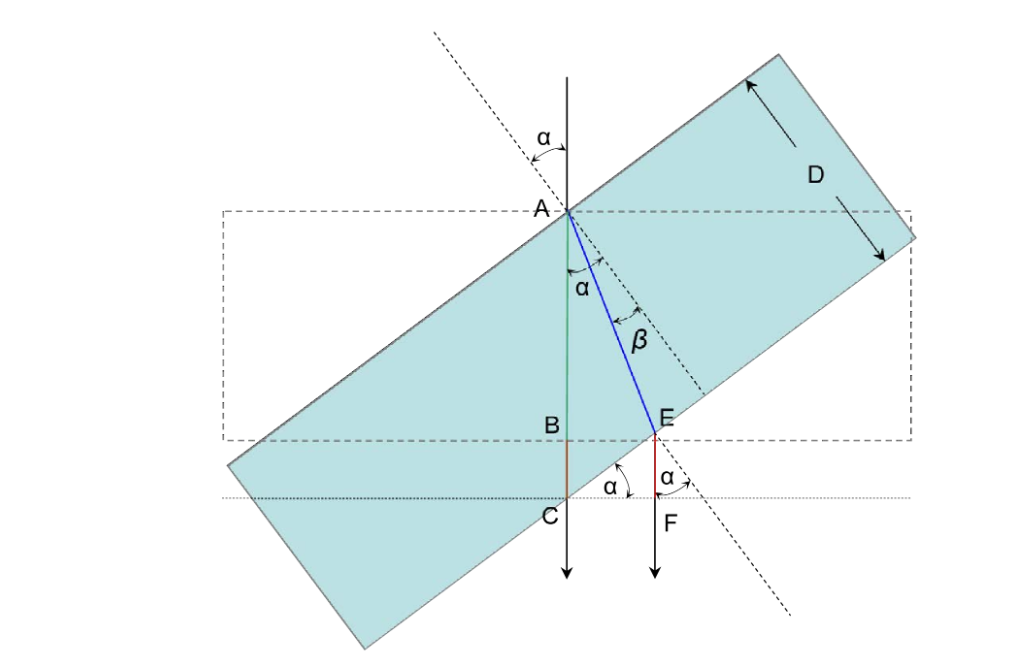
\includegraphics[width=1.0\textwidth]{images/Formula}
		\centering
		\caption{Skizze des Glas in zwei Zuständen: Einfallswinkel $\alpha= 0$ (gestrichelter Quader) und $\alpha>0$ (ausgefüllter Quader).\cite{GlasFormula}} %TODO gestrichelt fine? Quader/Quadrat %TODO cite right?
		\label{fig_glass_rotation}
		\centering
	\end{figure}

	Da sich das Glas in einem Arm des Michelson-Interferometers befindet, durchlaufen Strahlen dieses doppelt.
	Außerdem muss der Gangunterschied $\Delta$ ein vielfaches der Wellenlänge sein. Der Gangunterschied ist die Differenz der optischen Weglängen:
	\begin{equation}
		\Delta = m\lambda = 2 \cdot \left(\int_{\text{Weg} A \rightarrow F} \! n(s) \, \mathrm{d}s - \int_{\text{Weg} A \rightarrow C} \! n(s) \, \mathrm{d}s \right)
	\end{equation}
	Aus der Geometrie und den konstanten Brechungsindizes folgt
	\begin{equation}
		m\lambda = 2(n\cdot \overline{AE} + \overline{EF} - n \cdot \overline{AB} - \overline{BC}),
		\label{eq_glas_2}
	\end{equation}
	wobei $n$ der Brechungsindex des Glas ist und $n_\text{Luft}=1$ angenommen wird.

	Unmittelbar aus \cref{fig_glass_rotation} zu entnehmen sind
		$\overline{AB} = D$,
		$\overline{AE} = \frac{D}{\cos{\beta}}$,
		$\overline{AC} = \frac{D}{\cos{\alpha}}$,
		$\overline{BC} = \overline{AC} -D = \frac{D}{\cos{\alpha}}-D$,
		$\overline{EF} = \overline{CE} \cdot \sin{\alpha} = D\cdot (\tan{\alpha}-\tan{\beta})\cdot \sin{\alpha}$.
	Ersetzt man die Strecken und dividiert durch $2D$ in \cref{eq_glas_2} folgt:
	\begin{equation}
		\frac{m\lambda}{2D} = \frac{n}{\cos{\beta}} + \sin{\alpha}\tan{\alpha} - \sin{\alpha}\tan{\beta}-n  - \frac{1}{cos{\alpha}} +1
	\end{equation}
	Durch das Snelliusssche Brechungsgesetz $n \cdot \sin{\beta} = \sin{\alpha}$  ergibt sich mit $\cos{\beta}=\sqrt{1-\frac{\sin^2{\alpha}}{n^2}}$:
	\begin{equation}
		\frac{m\lambda}{2D} = \sqrt{n^2-\sin^2{\alpha}} -\cos{\alpha} - n + 1
	\end{equation}
	und quadriert
	\begin{equation}
		\left(\frac{m\lambda}{2D}+ \cos{\alpha}-1+n\right)^2 = n^2-\sin^2{\alpha}
	\end{equation}
	Nach Ausmultiplizieren und Umformen ergibt sich:
	\begin{equation}
		n=\frac{\sin^2{\alpha}+\left(\frac{m\lambda}{2D} + \cos{\alpha}-1\right)^2}{2(1-cos{\alpha}-\frac{m\lambda}{2D})}
	\end{equation}
	Mit $\alpha=\Phi$, und $D=t$ lässt sich dies in die Formel aus der Einführung umstellen:
	\begin{equation}
		n= \frac{(2t-m\lambda)(1-\cos{\Phi})+ \frac{m^2\lambda^2}{4t}}{2t(1-\cos{\Phi})-m\lambda}
		\label{eq_brechindex}
	\end{equation}

	\subsection{Bestimmung des Brechungsindex eines Gases durch Druckänderung}
	Die Bedingung für Interferenz lautet:
	\begin{equation}
		m\lambda = n_1 l - n_2 l
		\label{eq_tmp_1}
	\end{equation}
	Verändert man den Druck des Gases ändert sich auch der Brechungsindex $n_1$ und es folgt ein neuer Gangunterschied:
	\begin{equation}
		m'\lambda = n_1' l - n_2 l
		\label{eq_tmp_2}
	\end{equation}
	Dividiert man die Differenz von \cref{eq_tmp_1} und \cref{eq_tmp_2} durch $\Delta p$ ergibt sich:
	\begin{equation}
		\frac{\Delta n}{\Delta p} = \frac{\Delta m}{\Delta p} \cdot \frac{\lambda}{l}
		\label{eq_brech_druck}
	\end{equation}
	Der Brechungsindex $n$ hängt linear vom Druck $p$ ab:
	\begin{equation}
		n(p) = n(p=0) + \frac{\Delta n}{\Delta p} p
	\end{equation}
	Dieser Zusammenhang wird aus der Näherungsformel
	\begin{equation}
		\frac{n-1}{\rho} = r_G = \text{const}
	\end{equation}
	klar. Da sich $n = 1+ r_G \cdot \rho$ ergibt und unter Annahme eines idealen Gases, also $\rho \propto p$, folgt die Linearität.


	\section{Methoden}
	% Bilder von der Website klauen
	% einer will Präsens
	Es soll mit dem Michelson-Interferometer die Wellenlänge eines Helium-Neon-Lasers und die Brechungsindizes von Luft, Kohlenstoffdioxid und einer Glasplatte bestimmt werden.
	Dazu wird der Aufbau in \cref{fig_aufbau} verwendet.

	\begin{figure}[H]
		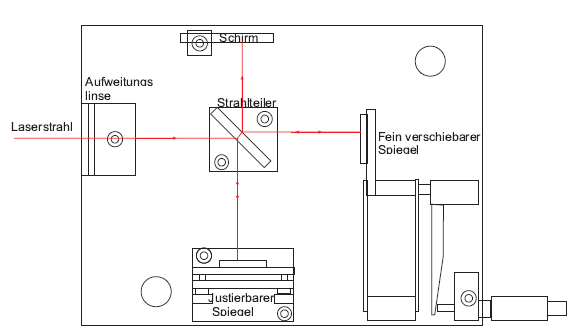
\includegraphics[width=\textwidth]{images/michelson_aufbau}
		\centering
		\caption{Aufbau des Michelson-Interferometers. \cite{Anleitung}}
		\label{fig_aufbau}
	\end{figure}

	Zunächst wird die Wellenlänge bestimmt, indem die Anzahl der durchlaufenden Interferenzringe $m$ auf dem Schirm in Abhängigkeit von der Verschiebung $\Delta s$ des fein verschiebbaren Spiegels gemessen wird. %TODO Laufende Ringe in Theorie
	Die Verschiebung wird mit einer Mikrometerschraube eingestellt und gemessen.
	Die Wellenlänge ergibt sich dann gemäß \cref{eq_wellenlaenge}.


	Dann wird in einen der Arme des Interferometers eine Glasplatte gebracht, die sich mit einer Mikrometerschraube kippen lässt. %TODO kp, ob Arm definiert ist als das, das zweimal durchlaufen wird.
	Hierbei wird zunächst die senkrechte Position gesucht, indem die Platte so lange gekippt wird, bis sich die Laufrichtung der Interferenzringe ändern.
	Mithilfe der Winkelskala an der Einfassung der Glasplatte wird dann das Verhältnis von Verstellung der Mikrometerschraube und Kippwinkel der Glasplatte bestimmt, indem die Schraube eine bestimmte Strecke herausgedreht wird und die Winkeländerung gemessen wird.
	Mithilfe von \cref{eq_brechindex} kann dann der Brechungsindex der Glasplatte bestimmt werden.
	Die Dicke der Glasplatte wird mit einer Schieblehre gemessen.

	Zuletzt wird die Glasplatte durch eine Küvette ersetzt, die nach Wahl evakuiert oder mit Luft oder Kohlenstoffdioxid gefüllt werden kann und deren Innendruck gemessen werden kann.
	Dieses Vorgehen basiert darauf, dass das Licht, dass durch den Küvettenarm läuft eine andere optische Weglänge zurücklegt, als das, welches durch den anderen Arm läuft.
	Es werden mehrere Messungen durchgeführt, bei denen die Küvette schrittweise evakuiert wird oder mit dem Gas gefüllt wird.
	Es wird nach jedem durchgelaufenen Interferenzring der aktuelle Druck in der Küvette gemessen, damit dann die Abhängigkeit des Brechungsindex vom Druck bestimmt werden kann.
	Die Länge der Küvette wird gemessen.

	\section{Ergebnisse und Diskussion}

	% Allgemeine Beobachtungen
	% Einflüsse von veränderten Parametern auf Messung

	% Berechung nach Aufgabenstellung
	\subsection{Bestimmung der Wellenlänge}
	\subsubsection{Beobachtung und Datenanalyse}
	Zur Bestimmung der Wellenlänge des Lasers wird der Spiegel an einem Arm des Michelson-Interferometers verschoben.
	In \cref{tb_lambda} ist die Anzahl der durchlaufenden Interferenzringe unter Verschiebung des Spiegels $\Delta s$ angegeben.
	Die Unsicherheit von $\Delta s$ setzt sich aus der der Mikrometerschraube $u_M=\SI{11}{nm}$ und der Genauigkeit mit welcher ein Interferenzmaximum lokalisiert wird, also dessen Breite $u_B=\SI{108}{nm}$. %TODO der Satz ist nicht verständlich %TODO schreiben was delta s ist
	Des Weiteren wird davon ausgegangen, dass man sich einmal verzählen kann.
	Es ergibt sich eine über die Messungen gemittelte Wellenlänge von \SI{650.4+-10.8}{nm}.

	\begin{table}[H]
		\centering
		\begin{tabular}{| c | c | c |}
			\hline
			  $m$ &  $\Delta s$ & $\lambda=2 \Delta s/m$\\ \hline
				25$\pm$0.3 & \SI{7905+-109}{nm} & \SI{632.4+-11.6}{nm}\\
				40$\pm$0.3& \SI{13085.1+-109}{nm} & \SI{654.3+-7.3}{nm}\\
				40$\pm$0.3& \SI{13289.7+-109}{nm} & \SI{664.5+-7.4}{nm}\\
				\hline
		\end{tabular}
		\caption{Die Anzahl der durchlaufenden Interferenzringe $m$ in Abhängigkeit von der Verschiebung des Spiegels $\Delta s$ an einem Michelson-Interferometer-Arm liefert die Wellenlänge $\lambda$ des Lasers gemäß \cref{eq_wellenlaenge}. }
		\label{tb_lambda}
	\end{table}


	\subsubsection{Diskussion}
	%TODO erstaunlich hohe schwankung imo

	Da ein Helium-Neon-Laser verwendet wird, ist zu erwarten, dass mit dem Michelson-Interferometer dessen charakteristische Wellenlänge von \SI{633}{nm} gemessen werden kann.
	Innerhalb der dopplten Unsicherheit kann dies mit dem gemessenen Mittelwert von \SI{650,4\pm 10,8}{nm} bestätigt werden.
	Bei Betrachtung von \cref{tb_lambda} ist festzustellen, dass die Messung von mehr durchlaufenden Interferenzringen eine Abweichung nach oben zur Folge hat, weshalb die Abweichung auf ein Übersehen eines Interferenzringes durch Zuweitdrehen der Mikrometerschraube zurückgeführt werden kann.

	\subsection{Bestimmung des Brechungsindex der Glasplatte}
	\subsubsection{Beobachtung und Datenanalyse}
	Zur Bestimmung des Brechungsindex der Glasplatte lässt sich \cref{eq_brechindex} umformen:
	\begin{equation}
		(1-\cos{\phi}) = \frac{nm\lambda+\frac{m^2\lambda^2}{4t}}{m\lambda+2t(n-1)}
		\label{eq_winkel_theo}
	\end{equation}
	Dabei ist $t= \SI{5.05+-0.05}{mm}$ die Dicke der Glasplatte.
	Die Messung dieser ist aufgrund ihere Einfassung erschwert, weshalb die Dicke der Einfassung gemessen wird und dann auf beiden Seiten die Differenz zwischen Glas und Einfassung subtrahiert wird.
	Die Unsicherheit beim Einstellen des Kippwinkels $\Phi$ über die Mikrometerschraube beträgt \SI{0.011}{\degree}.
	In \cref{fig_glas} sind die mit $(1-\cos{\Phi})$ transformierten Messpunkte sowie ein Fit gemäß \cref{eq_winkel_theo} dargestellt.
	Der Fit liefert einen Brechungsindex von \SI{1.707+-0.013}{} für die Glasplatte für eine Wellenlänge $\lambda$ von \SI{650.4+-10.8}{nm}.

\begin{figure}[H]
		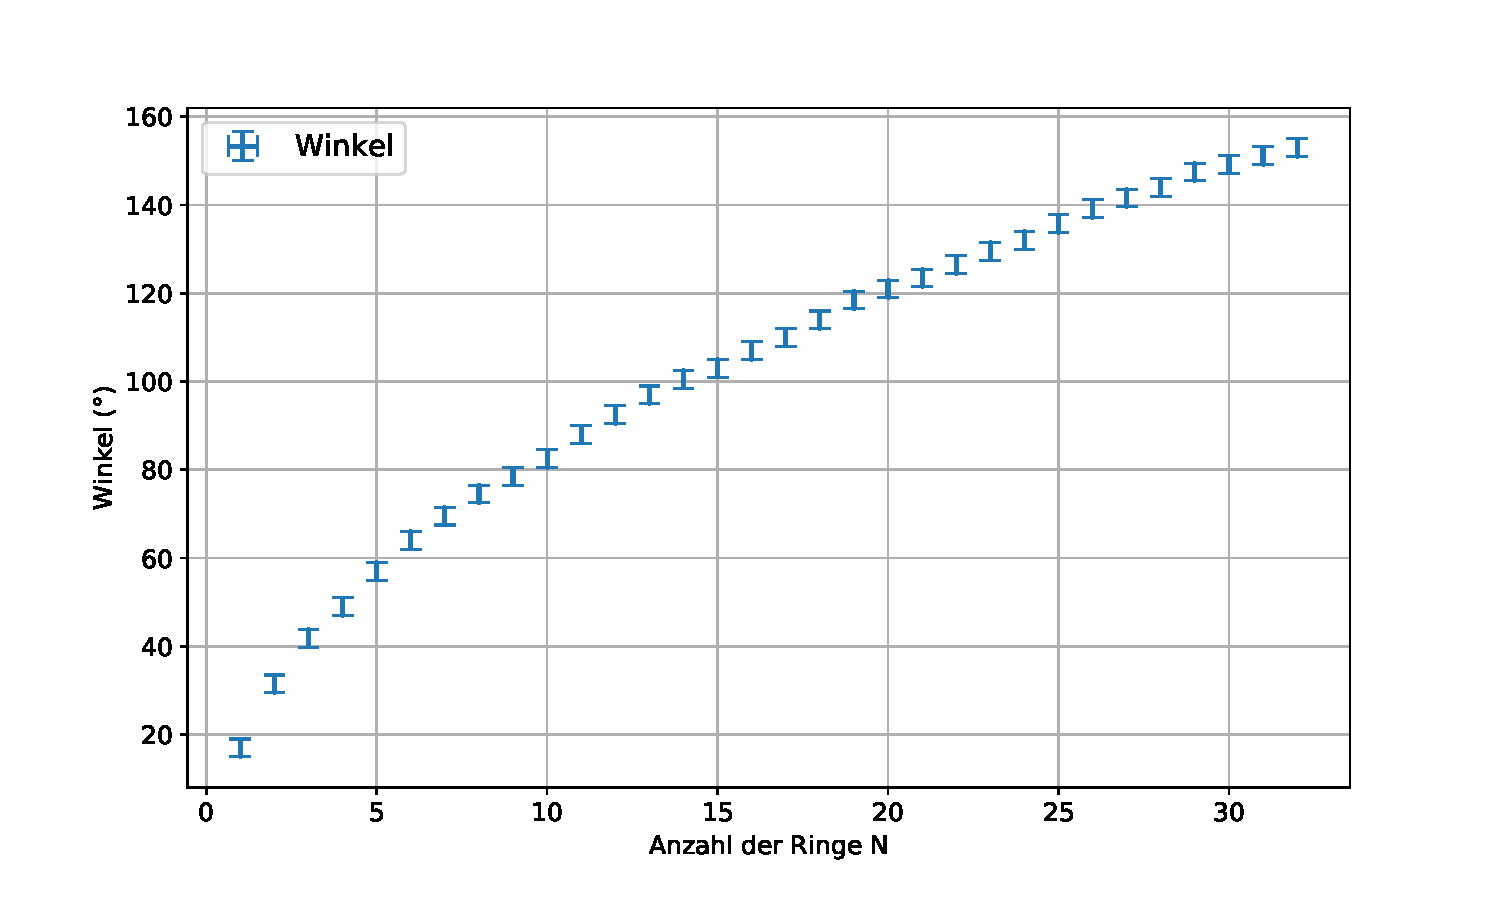
\includegraphics[width=\textwidth]{images/Glas.pdf}
		\centering
		\caption{Der Winkel der Glasplatte ist gegen die Änderung der Interferenzringe auf getragen.
		Die gelbe Funktion ist ein Fit gemäß den theoretischen erwarteten \cref{eq_winkel_theo}.}
		\label{fig_glas}
	\end{figure}

	\subsubsection{Diskussion}
	Da nicht bekannt ist, um welches Glas es sich bei der untersuchten Platte hält, ist es nicht möglich den Messwert anhand eines Literaturwertes zu prüfen.
	Es lässt sich allerdings sagen, dass der Messwert von \SI{1.707+-0.013}{nm} inerhalb des Bereichs von Brechungsindizes üblicher Gläser liegt.
	So hat zum Beispiel N-BAF10-Glas einen Brechungsindex von \SI{1,6661}{} bei einer Wellenlänge von \SI{650}{nm}.\cite{Brechungsindizes}

	\subsection{Bestimmung der Brechungsindizes von Gasen}
	\subsubsection{Beobachtung und Datenanalyse}
	Der Brechungsindex des jeweiligen Gases ist linear druckabhängig:
	\begin{equation}
		n(p) = n(p=0) + \frac{\Delta n}{\Delta p}p
		\label{eq_brech_p}
	\end{equation}
	Der Brechungsindex im Vakuum $n(p=0)$ beträgt 1.
	Die Abhängigkeit des Brechungsindexes vom Druck wird durch \cref{eq_brech_druck} beschrieben, hierbei ist zu beachten, dass die Küvette zweimal von dem Strahl durchlaufen wird:
	\begin{equation}
			\frac{\Delta n}{\Delta p} = \frac{\Delta m}{\Delta p} \frac{\lambda}{2l}
	\end{equation}

	Wobei $l=\SI{3.5+-0.3}{cm}$ die Länge der Küvette im Strahlengang ist, welche abgeschätzt werden musste, da die Innenlänge des Behälters nicht bekannt ist.
	Die Unsicherheit des Präzisions-Digital-Grobvakuummeters beträgt \SI{0.3}{mbar} und die Wellenlänge des Lasers beträgt nach wie vor \SI{650.4+-10.8}{nm}.

	In \crefrange{fig_luft_raus}{fig_co2_rein} ist der Druck $p$ gegen die Anzahl der Interferenzringe $m$ aufgetragen und es wurden lineare Fits durchgeführt, um $\Delta p / \Delta m$ und somit den Kehrwert $\Delta m / \Delta p$ zu ermitteln.
	Dabei ist zu beachten, dass sich bei inverser Druckänderung auch die Interferenzringe in die umgekehrte Richtung verschieben, die Quotienten haben folglich immer das gleiche Vorzeichen.
	In \cref{tb_gase} sind die aus den Fitparameter resultierenden Brechungsindizes der Gase aufgelistet.

\begin{figure}[H] %TODO ist imo noch nicht ANhang worthy
		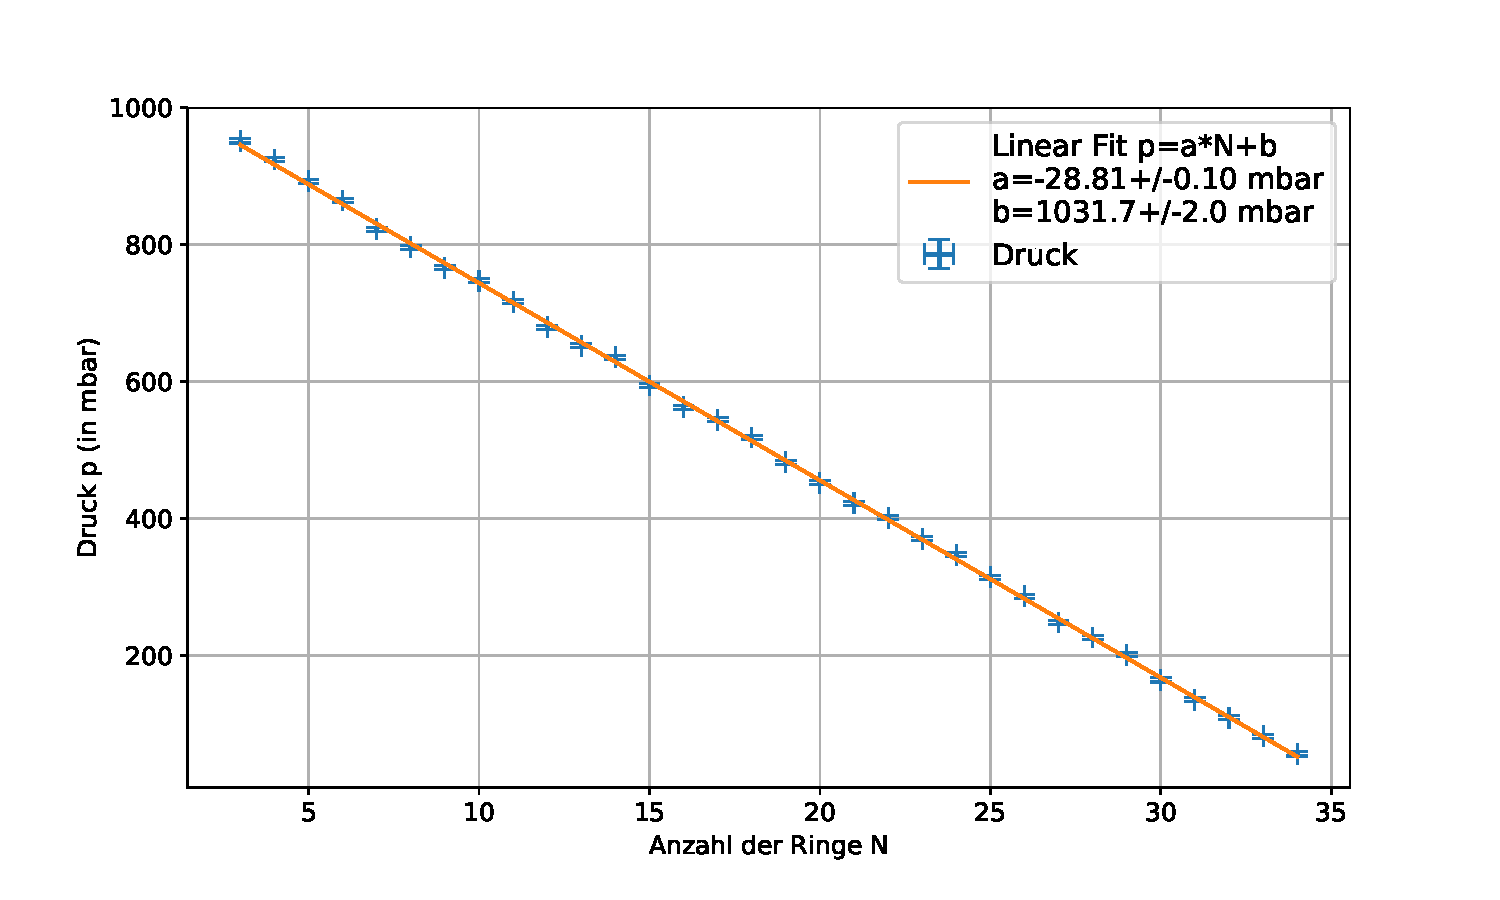
\includegraphics[width=0.9\textwidth]{images/Luft_Raus.pdf}
		\centering
		\caption{In der Küvette befindet sich Luft. Der Druck wird kontinuierlich reduziert. Die gelbe Funktion ist ein linearer Fit.}
		\label{fig_luft_raus}
	\end{figure}
\begin{figure}[H]
		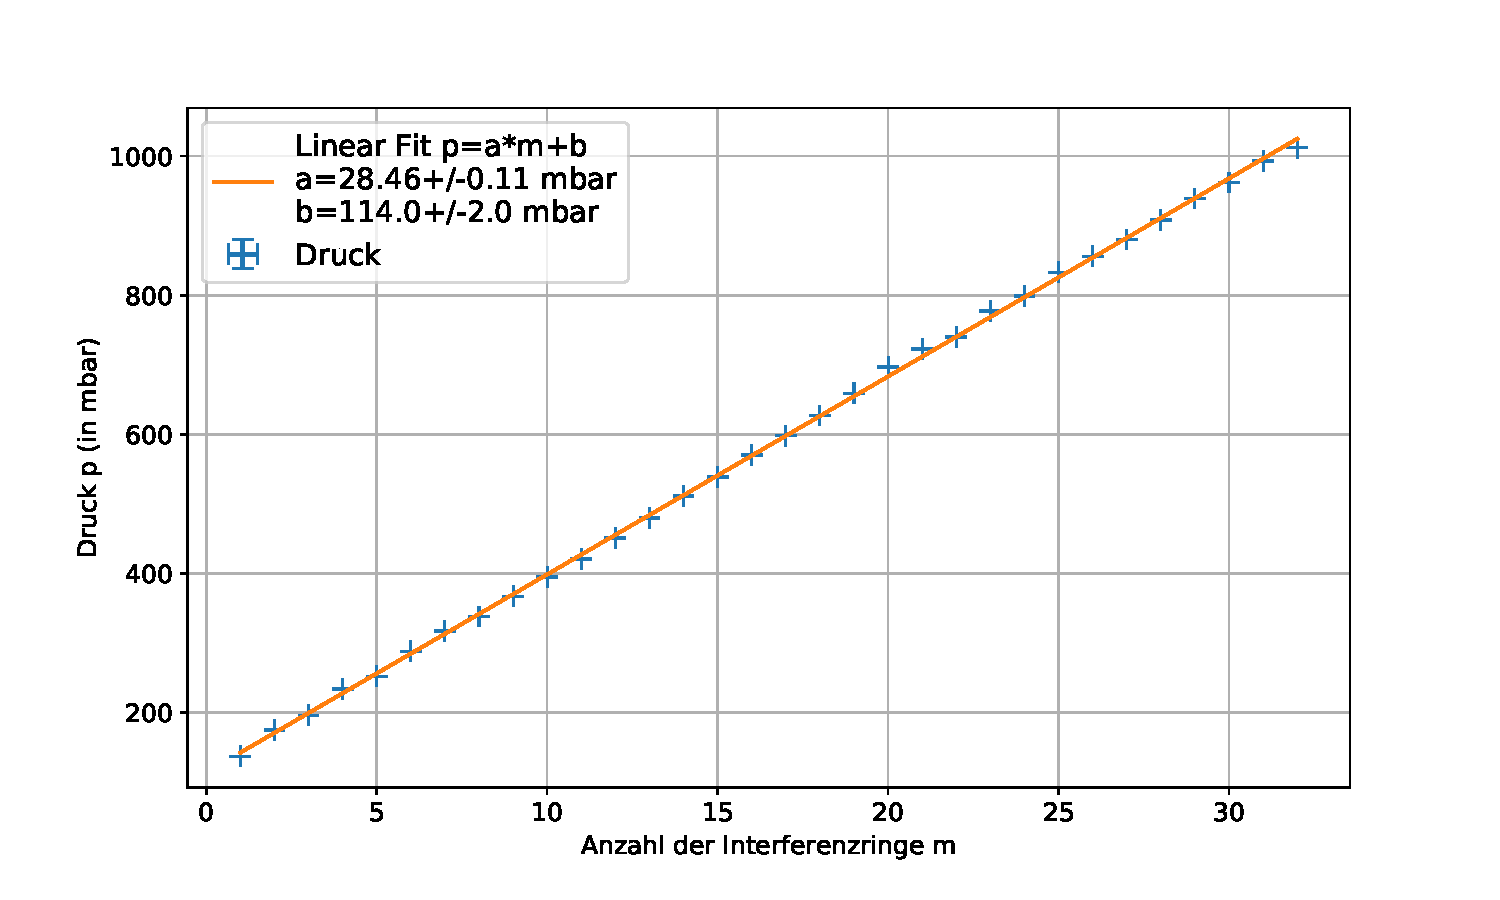
\includegraphics[width=0.9\textwidth]{images/Luft_Rein.pdf}
		\centering
		\caption{In der Küvette befindet sich Luft. Der Druck wird kontinuierlich erhöht. Die gelbe Funktion ist ein linearer Fit.}
		\label{fig_luft_rein}
	\end{figure}
\begin{figure}[H]
		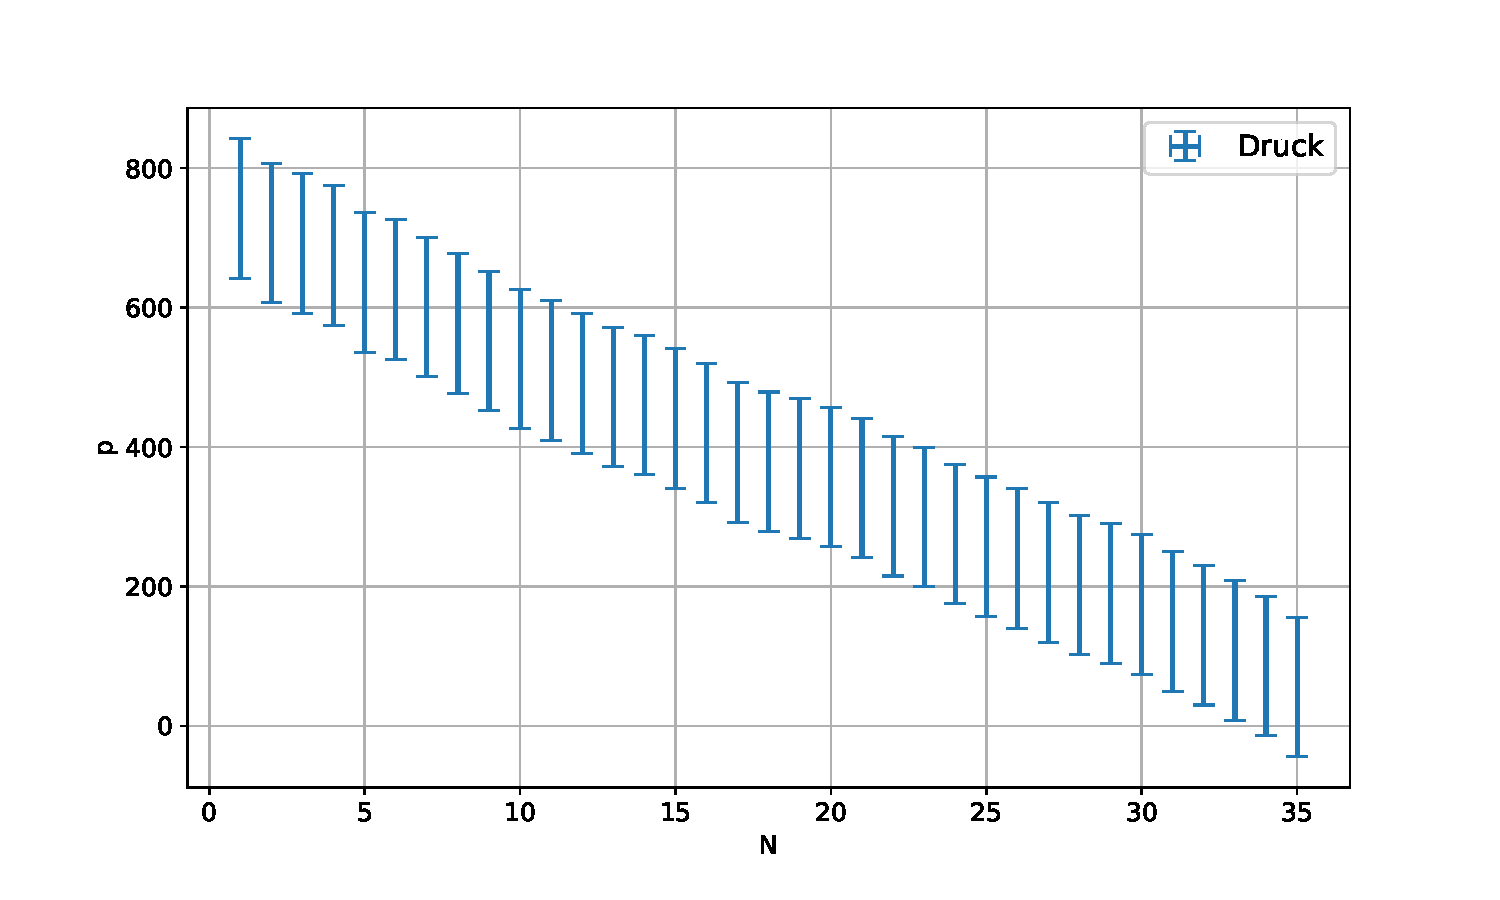
\includegraphics[width=0.9\textwidth]{images/CO2_Raus.pdf}
		\centering
		\caption{In der Küvette befindet sich CO$_2$. Der Druck wird kontinuierlich reduziert. Die gelbe Funktion ist ein linearer Fit.}
		\label{fig_co2_raus}
	\end{figure}
\begin{figure}[H]
		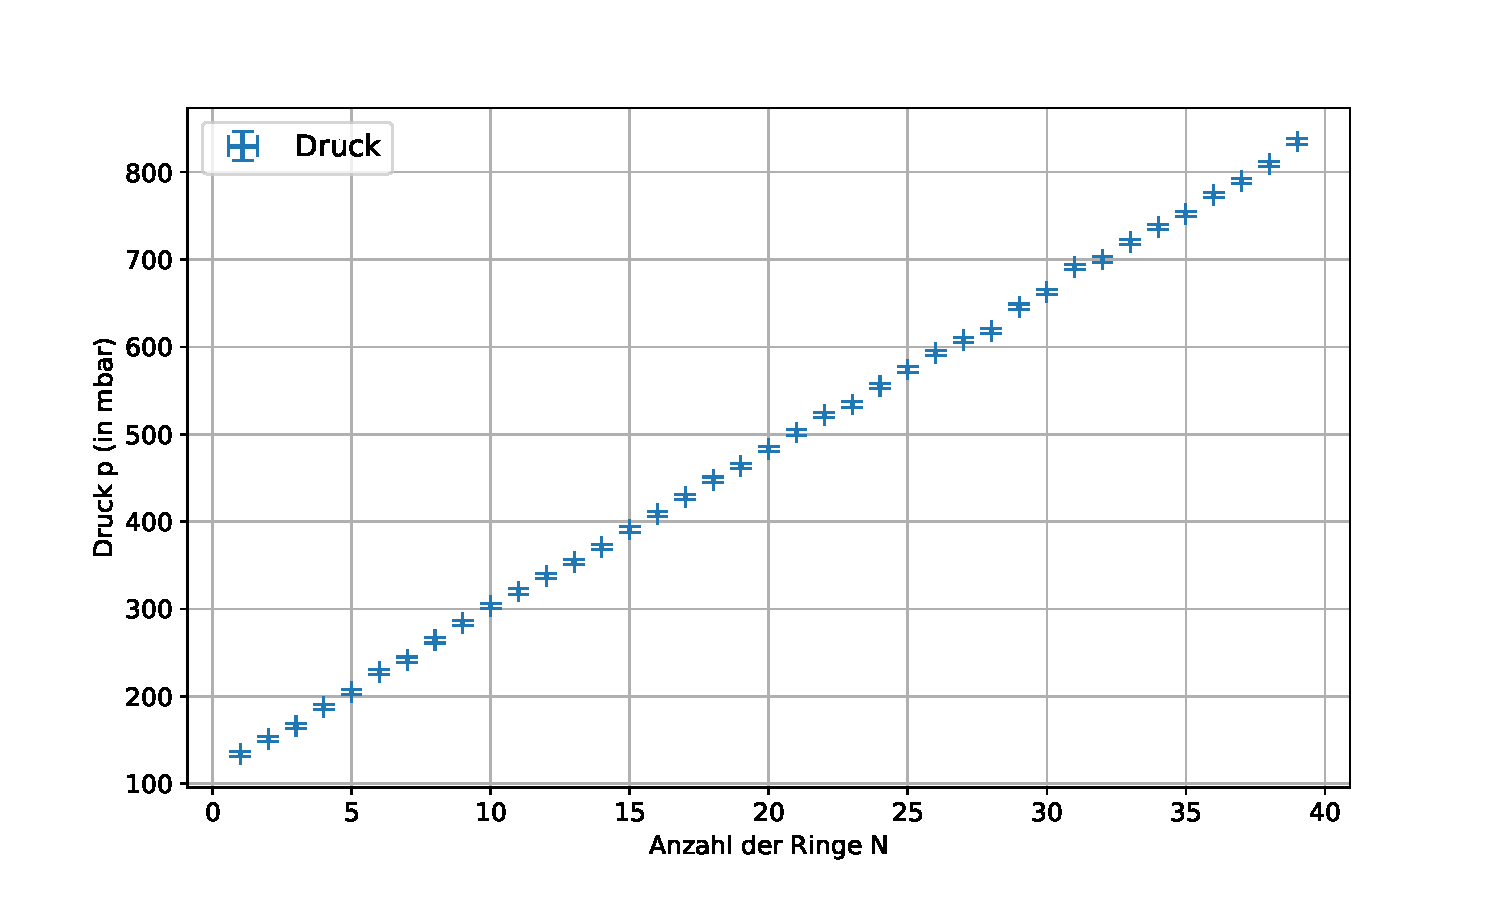
\includegraphics[width=0.9\textwidth]{images/CO2_Rein.pdf}
		\centering
		\caption{In der Küvette befindet sich CO$_2$. Der Druck wird kontinuierlich erhöht. Die gelbe Funktion ist ein linearer Fit.}
		\label{fig_co2_rein}
	\end{figure}



	\begin{table}[H]
		\centering
		\begin{tabular}{| c | c | c |}
			\hline
			  Gas &  $\Delta p/\Delta m$ & $n(p=\SI{1013}{mbar})$\\ \hline
				Luft& \SI{28.81+-0.1}{mbar} & \SI{1.000327+-0.000029}{}\\
				&\SI{28.46+-0.11}{mbar}&\SI{1.000331+-0.000029}{}\\
				CO$_2$ & \SI{19.11+-0.18}{mbar} & \SI{1.000493+-0.000043}{}\\
				&\SI{18.28+-0.04}{mbar}&\SI{1.000514+-0.000045}{}\\
				\hline
		\end{tabular}
		\caption{Die Brechungsindizes bei Normaldruck werden aus den durchlaufenden Interferenzringen pro Druckänderung mit \cref{eq_brech_p} bestimmt.} %TODO in tabelle welches steigt und welches abfällt? %TODO besserer Text
		\label{tb_gase}
	\end{table}


	Für die Brechungsindizes ergeben sich mit gemittelten Steigungen abhängig vom Druck $p$:

	\begin{equation}
		n_\text{Luft}(p) = 1+p \cdot \SI{3.24+-0.28e-7}{mbar^{-1}}
	\end{equation}
	\begin{equation}
		n_\text{CO$_2$}(p) = 1+ p \cdot \SI{4.97+-0.44e-7}{mbar^{-1}}
	\end{equation}
	\subsubsection{Diskussion}
	% Bezug/Nutzen oder sonst was
	% auch hier die Hypothese wiederholen
	% keine Messwerte hier, nach manchen Menschen, zumindest "direkt" erstellte Diagramme net hier, auch wenn Lesbarkeit-bla
	%TODO siehe Kurzfassung
	%TODO Temperatur hat Einfluss, thermo dyn. Prozesse relevant? (adiabatisch o.ä.?)
	%TODO geringe Schwankungen bei kontinuierlichem Messen sind ziemlich ahnbar
	%TODO rein ca. gleich wie raus erwartbar
	%TODO qualitativ passt es und quantitativ vmtl. auch
	Zunächst lässt sich sagen, dass anhand von \crefrange{fig_luft_raus}{fig_co2_rein} der lineare Zusammenhang aus \cref{eq_brech_p} bestätigen lässt.
	Die Abweichungen vom Fit liegen im Wesentlichen innerhalb der doppelten Unsicherheit und sind darauf zurückzuführen, dass die Gaszuführ bzw. Evakuierung nicht nach jedem durchgelaufenen Interferenzring an der selben Position der Ringe gestoppt werden kann.
	Außerdem kann anhand von \cref{tb_gase} festgestellt werden, dass die Messung von $\Delta p/\Delta m$ bei Werte Zufuhr bzw. Abfuhr des Gases ähnliche Messwerte ergeben, deren doppelten Unsicherheitsintervalle allerdings nur im Fall von Luft überschneiden.
	Der Grund für die Abweichung bei CO$_2$ liegt vermutlich im Übersehen eines Interferenzrings bei zu schneller Gaszufuhr bzw. Evakuierung.

	Der Messwert bei Atmosphärendruck lässt sich einfach mit Literaturwerten bei einer Wellenlänge von \SI{650}{nm} vergleichen.
	Für Luft ist hier ein Wert von \SI{1.00027632}{} zu erwarten (vgl. \cite{Brechungsindizes}).
	Die liegt erwartungsgemäß innerhalb der doppelten Unsicherheit der Messwerte aus \cref{tb_gase}.

	Für Kohlenstoffdioxid wird gemäß \cite{GlasFormula} ein Wert von \SI{1.00044727}{} erwartet und auch dies liegt innerhalb der doppelten Unsicherheit der Messwerte.

	\section{Schlussfolgerung}
	% Rückgriff auf Hypothese und drittes Nennen dieser
	Insgesamt lässt sich sagen, dass die zu untersuchenden Material- bzw. Lasereigenschaften gemessen werden konnten, ohne dabei den Erwartungen zu widersprechen.
	Zunächst wurde die Wellenlänge des Lasers bestimmt, was Übereinstimmung mit der Tatsache, dass es sich um einen Helium-Neon-Laser handelte, ergab.
	Dann wurde der Brechungsindex einer Glasscheibe durch schrittweises Kippen dieser bestimmt.
	Zuletzt wurde die Druckabhängigkeit der Brechungsindizes von Luft und Kohlenstoffdioxid bestimmt, wobei die angenommene Linearität bestätig werden kann.
	Es lässt sich also feststellen, dass das Michelson-Interferometer tatsächlich ein valides Mittel für diese Untersuchungen ist. %TODO zu cheesy?

	% Quellen zitieren, Websiten mit Zugriffsdatum
	% Verweise auf das Laborbuch (sind erlaubt)
	% Tabelle + Bilder mit Beschriftung
	\printbibliography
\end{document}
